\begin{figure}[H]
    \centering
    \begin{tikzpicture}[]
        \pgfplotsset{
            width=0.4\textwidth,
            height=0.4\textheight
        }
        \begin{axis}[
            xlabel={DEC Consumption (Joules)}, 
            ylabel={Measurements}, 
            title={The evolution of energy consumption}, 
            ytick={1, 2, 3, 4, 5, 6, 7, 8, 9, 10, 11, 12, 13, 14, 15},
        yticklabels={
            200, 400, 600, 800, 1000, 1200, 1400, 1600, 1800, 2000, 2200, 2400, 2600, 2800, 3000, 
            },
            xmin=400,xmax=900,
            ]
        
        
        \addplot+ [boxplot prepared={
                lower whisker=696.3949814185205,
                lower quartile=738.8897176884595,
                median=757.8874784997041,
                upper quartile=771.0083916802237,
                upper whisker=813.27407546102
                }, color = red
                ] coordinates{(0,555.0410025879717)(0,588.4977116550981)(0,608.0868646883634)(0,592.3173001802113)(0,614.076889339419)(0,617.6992020041132)(0,602.3264998972172)(0,585.5616563721271)(0,623.3135003704065)(0,636.1142739282798)(0,591.4449723057328)(0,579.022257899517)(0,670.4168666339185)(0,623.4922094737083)(0,820.5957514537629)};
        
        \addplot+ [boxplot prepared={
                lower whisker=696.3949814185205,
                lower quartile=743.6241548341852,
                median=762.6801093811176,
                upper quartile=776.3994624386503,
                upper whisker=823.8241291582406
                }, color = red
                ] coordinates{(1,555.0410025879717)(1,588.4977116550981)(1,608.0868646883634)(1,592.3173001802113)(1,614.076889339419)(1,617.6992020041132)(1,602.3264998972172)(1,585.5616563721271)(1,623.3135003704065)(1,636.1142739282798)(1,591.4449723057328)(1,579.022257899517)(1,670.4168666339185)(1,623.4922094737083)(1,609.5474823042591)(1,601.3934403280459)(1,620.4452795868222)(1,640.667350654579)(1,636.8090350140501)(1,621.6286750157569)(1,658.3638158219683)(1,618.4796403355831)(1,659.3363880460233)(1,619.3110920261774)(1,636.5570561819025)(1,600.4914636963811)(1,620.3261420342462)(1,587.8394302072363)(1,606.7385964851685)(1,611.3760730395973)(1,606.5917147286107)(1,594.4676635141784)(1,832.929192296567)(1,839.8119703912428)(1,826.8709977855838)};
        
        \addplot+ [boxplot prepared={
                lower whisker=654.6024612042527,
                lower quartile=720.2423372213295,
                median=747.1625894202339,
                upper quartile=767.9263931253331,
                upper whisker=832.929192296567
                }, color = red
                ] coordinates{(2,555.0410025879717)(2,588.4977116550981)(2,608.0868646883634)(2,592.3173001802113)(2,614.076889339419)(2,617.6992020041132)(2,602.3264998972172)(2,585.5616563721271)(2,623.3135003704065)(2,636.1142739282798)(2,591.4449723057328)(2,579.022257899517)(2,623.4922094737083)(2,609.5474823042591)(2,601.3934403280459)(2,620.4452795868222)(2,640.667350654579)(2,636.8090350140501)(2,621.6286750157569)(2,618.4796403355831)(2,619.3110920261774)(2,636.5570561819025)(2,600.4914636963811)(2,620.3261420342462)(2,587.8394302072363)(2,606.7385964851685)(2,611.3760730395973)(2,606.5917147286107)(2,594.4676635141784)(2,584.4792725008563)(2,591.2103631697751)(2,570.510785737845)(2,576.3671081090763)(2,614.9116958343741)(2,605.8828498591288)(2,587.861206395748)(2,561.0588363551221)(2,578.8350187417452)(2,560.877361822714)(2,574.5066271788287)(2,570.1151460991894)(2,552.3828782997334)(2,552.11255606131)(2,565.2747041129451)(2,565.7330394559435)(2,564.2534515243867)(2,565.1932277516123)(2,580.6022633093676)(2,839.8119703912428)};
        
        \addplot+ [boxplot prepared={
                lower whisker=565.7330394559435,
                lower quartile=683.9916138575175,
                median=733.1299553903067,
                upper quartile=762.915061924816,
                upper whisker=839.8119703912428
                }, color = red
                ] coordinates{(3,555.0410025879717)(3,561.0588363551221)(3,560.877361822714)(3,552.3828782997334)(3,552.11255606131)(3,565.2747041129451)(3,564.2534515243867)(3,565.1932277516123)(3,528.4667361894719)(3,546.9851154920555)(3,548.9577319003652)(3,546.0289030294775)(3,553.3576966232931)(3,549.5885368610066)(3,536.5083253504658)(3,560.0957621303023)(3,528.9191097696571)(3,562.6472615898076)(3,554.4889672382158)(3,565.5559976638033)(3,552.1365368761988)(3,510.2579671342785)(3,541.980568201489)(3,543.8432695252554)(3,537.2838884039088)(3,538.0610937749664)(3,529.0494077840181)(3,545.8933798773921)(3,513.6752281536644)(3,539.6855793994307)(3,542.1713667119816)(3,542.1713667119816)(3,542.1713667119816)(3,548.9069735747323)(3,543.2728646388014)(3,537.5673830559781)(3,532.573345405709)(3,502.3989876698695)(3,545.8312683443992)(3,546.9897174040191)(3,528.9474827134607)(3,539.1327691487616)(3,541.5199860217638)(3,522.2569005937582)(3,532.0482359298051)};
        
        \addplot+ [boxplot prepared={
                lower whisker=541.3563369655199,
                lower quartile=669.8595151966014,
                median=715.7500085866907,
                upper quartile=755.6106323698957,
                upper whisker=839.8119703912428
                }, color = red
                ] coordinates{(4,528.4667361894719)(4,536.5083253504658)(4,528.9191097696571)(4,510.2579671342785)(4,537.2838884039088)(4,538.0610937749664)(4,529.0494077840181)(4,513.6752281536644)(4,539.6855793994307)(4,537.5673830559781)(4,532.573345405709)(4,502.3989876698695)(4,528.9474827134607)(4,539.1327691487616)(4,522.2569005937582)(4,532.0482359298051)(4,499.78265645599413)(4,507.7950915663341)(4,520.0267655883945)(4,510.57195091700555)(4,515.8478042868039)(4,536.7777057593826)(4,524.3622157229561)(4,531.6454347564943)(4,529.013399250721)(4,539.3173841390612)};
        
        \addplot+ [boxplot prepared={
                lower whisker=553.3576966232931,
                lower quartile=676.2625528031938,
                median=725.5957275117507,
                upper quartile=758.7308157556452,
                upper whisker=839.8119703912428
                }, color = red
                ] coordinates{(5,552.3828782997334)(5,552.11255606131)(5,528.4667361894719)(5,546.9851154920555)(5,548.9577319003652)(5,546.0289030294775)(5,549.5885368610066)(5,536.5083253504658)(5,528.9191097696571)(5,552.1365368761988)(5,510.2579671342785)(5,541.980568201489)(5,543.8432695252554)(5,537.2838884039088)(5,538.0610937749664)(5,529.0494077840181)(5,545.8933798773921)(5,513.6752281536644)(5,539.6855793994307)(5,542.1713667119816)(5,542.1713667119816)(5,542.1713667119816)(5,548.9069735747323)(5,543.2728646388014)(5,537.5673830559781)(5,532.573345405709)(5,502.3989876698695)(5,545.8312683443992)(5,546.9897174040191)(5,528.9474827134607)(5,539.1327691487616)(5,541.5199860217638)(5,522.2569005937582)(5,532.0482359298051)(5,499.78265645599413)(5,507.7950915663341)(5,520.0267655883945)(5,510.57195091700555)(5,515.8478042868039)(5,536.7777057593826)(5,550.1864844675961)(5,524.3622157229561)(5,531.6454347564943)(5,552.1631006790446)(5,529.013399250721)(5,547.2814965251544)(5,541.3563369655199)(5,539.3173841390612)};
        
        \addplot+ [boxplot prepared={
                lower whisker=560.877361822714,
                lower quartile=680.2824625213713,
                median=730.1140904742722,
                upper quartile=759.9276842500594,
                upper whisker=839.8119703912428
                }, color = red
                ] coordinates{(6,555.0410025879717)(6,552.3828782997334)(6,552.11255606131)(6,528.4667361894719)(6,546.9851154920555)(6,548.9577319003652)(6,546.0289030294775)(6,553.3576966232931)(6,549.5885368610066)(6,536.5083253504658)(6,560.0957621303023)(6,528.9191097696571)(6,554.4889672382158)(6,552.1365368761988)(6,510.2579671342785)(6,541.980568201489)(6,543.8432695252554)(6,537.2838884039088)(6,538.0610937749664)(6,529.0494077840181)(6,545.8933798773921)(6,513.6752281536644)(6,539.6855793994307)(6,542.1713667119816)(6,542.1713667119816)(6,542.1713667119816)(6,548.9069735747323)(6,543.2728646388014)(6,537.5673830559781)(6,532.573345405709)(6,502.3989876698695)(6,545.8312683443992)(6,546.9897174040191)(6,528.9474827134607)(6,539.1327691487616)(6,541.5199860217638)(6,522.2569005937582)(6,532.0482359298051)(6,499.78265645599413)(6,507.7950915663341)(6,520.0267655883945)(6,510.57195091700555)(6,515.8478042868039)(6,536.7777057593826)(6,550.1864844675961)(6,556.4062353227255)(6,524.3622157229561)(6,531.6454347564943)(6,552.1631006790446)(6,529.013399250721)(6,559.040545167449)(6,547.2814965251544)(6,541.3563369655199)(6,556.1311874446037)(6,539.3173841390612)(6,560.0575044477996)};
        
        \addplot+ [boxplot prepared={
                lower whisker=564.2534515243867,
                lower quartile=678.9482932366661,
                median=721.337733333111,
                upper quartile=756.052991952007,
                upper whisker=839.8119703912428
                }, color = red
                ] coordinates{(7,555.0410025879717)(7,561.0588363551221)(7,560.877361822714)(7,552.3828782997334)(7,552.11255606131)(7,528.4667361894719)(7,546.9851154920555)(7,548.9577319003652)(7,546.0289030294775)(7,553.3576966232931)(7,549.5885368610066)(7,536.5083253504658)(7,560.0957621303023)(7,528.9191097696571)(7,562.6472615898076)(7,554.4889672382158)(7,552.1365368761988)(7,510.2579671342785)(7,541.980568201489)(7,543.8432695252554)(7,537.2838884039088)(7,538.0610937749664)(7,529.0494077840181)(7,545.8933798773921)(7,513.6752281536644)(7,539.6855793994307)(7,542.1713667119816)(7,542.1713667119816)(7,542.1713667119816)(7,548.9069735747323)(7,543.2728646388014)(7,537.5673830559781)(7,532.573345405709)(7,502.3989876698695)(7,545.8312683443992)(7,546.9897174040191)(7,528.9474827134607)(7,539.1327691487616)(7,541.5199860217638)(7,522.2569005937582)(7,532.0482359298051)(7,499.78265645599413)(7,507.7950915663341)(7,520.0267655883945)(7,510.57195091700555)(7,515.8478042868039)(7,536.7777057593826)(7,550.1864844675961)(7,556.4062353227255)(7,524.3622157229561)(7,531.6454347564943)(7,552.1631006790446)(7,529.013399250721)(7,559.040545167449)(7,547.2814965251544)(7,541.3563369655199)(7,556.1311874446037)(7,539.3173841390612)(7,560.0575044477996)(7,559.3165086195745)(7,561.3568000672574)(7,562.0219110364869)(7,545.8552800271555)(7,541.8831662858711)(7,547.637646271022)(7,551.2015196500413)(7,537.3268805435225)(7,554.784027827669)(7,546.1637721806064)(7,548.5543720125809)(7,557.3390069378504)(7,551.1570421022805)(7,557.0369602285184)(7,540.7721973528576)(7,535.488754171244)(7,530.928824078353)(7,541.2355432339928)};
        
        \addplot+ [boxplot prepared={
                lower whisker=559.040545167449,
                lower quartile=674.4765553579655,
                median=715.1408268087886,
                upper quartile=751.7731693988926,
                upper whisker=839.8119703912428
                }, color = red
                ] coordinates{(8,555.0410025879717)(8,552.3828782997334)(8,552.11255606131)(8,528.4667361894719)(8,546.9851154920555)(8,548.9577319003652)(8,546.0289030294775)(8,553.3576966232931)(8,549.5885368610066)(8,536.5083253504658)(8,528.9191097696571)(8,554.4889672382158)(8,552.1365368761988)(8,510.2579671342785)(8,541.980568201489)(8,543.8432695252554)(8,537.2838884039088)(8,538.0610937749664)(8,529.0494077840181)(8,545.8933798773921)(8,513.6752281536644)(8,539.6855793994307)(8,542.1713667119816)(8,542.1713667119816)(8,542.1713667119816)(8,548.9069735747323)(8,543.2728646388014)(8,537.5673830559781)(8,532.573345405709)(8,502.3989876698695)(8,545.8312683443992)(8,546.9897174040191)(8,528.9474827134607)(8,539.1327691487616)(8,541.5199860217638)(8,522.2569005937582)(8,532.0482359298051)(8,499.78265645599413)(8,507.7950915663341)(8,520.0267655883945)(8,510.57195091700555)(8,515.8478042868039)(8,536.7777057593826)(8,550.1864844675961)(8,556.4062353227255)(8,524.3622157229561)(8,531.6454347564943)(8,552.1631006790446)(8,529.013399250721)(8,547.2814965251544)(8,541.3563369655199)(8,556.1311874446037)(8,539.3173841390612)(8,545.8552800271555)(8,541.8831662858711)(8,547.637646271022)(8,551.2015196500413)(8,537.3268805435225)(8,554.784027827669)(8,546.1637721806064)(8,548.5543720125809)(8,557.3390069378504)(8,551.1570421022805)(8,557.0369602285184)(8,540.7721973528576)(8,535.488754171244)(8,530.928824078353)(8,541.2355432339928)(8,519.3583678554951)(8,529.6348975335945)(8,522.2775850612461)(8,522.1933176904445)(8,538.0188667662287)(8,530.5160209342196)(8,533.0126657199462)(8,522.9994381132892)(8,517.4734602520489)(8,516.4687430603558)(8,509.39032292412867)(8,510.9159225931144)(8,529.1131927601018)(8,541.9828604620659)(8,521.622715710612)(8,548.8904614821647)(8,549.4623593350727)(8,557.1412877177172)(8,550.266223044249)};
        
        \addplot+ [boxplot prepared={
                lower whisker=570.1151460991894,
                lower quartile=676.8001678033734,
                median=713.7983906661005,
                upper quartile=748.0621060159599,
                upper whisker=839.8119703912428
                }, color = red
                ] coordinates{(9,555.0410025879717)(9,561.0588363551221)(9,560.877361822714)(9,552.3828782997334)(9,552.11255606131)(9,565.2747041129451)(9,565.7330394559435)(9,564.2534515243867)(9,565.1932277516123)(9,528.4667361894719)(9,546.9851154920555)(9,548.9577319003652)(9,546.0289030294775)(9,553.3576966232931)(9,549.5885368610066)(9,536.5083253504658)(9,560.0957621303023)(9,528.9191097696571)(9,562.6472615898076)(9,554.4889672382158)(9,565.5559976638033)(9,552.1365368761988)(9,510.2579671342785)(9,541.980568201489)(9,543.8432695252554)(9,537.2838884039088)(9,538.0610937749664)(9,529.0494077840181)(9,545.8933798773921)(9,513.6752281536644)(9,539.6855793994307)(9,542.1713667119816)(9,542.1713667119816)(9,542.1713667119816)(9,548.9069735747323)(9,543.2728646388014)(9,537.5673830559781)(9,532.573345405709)(9,502.3989876698695)(9,545.8312683443992)(9,546.9897174040191)(9,528.9474827134607)(9,539.1327691487616)(9,541.5199860217638)(9,522.2569005937582)(9,532.0482359298051)(9,499.78265645599413)(9,507.7950915663341)(9,520.0267655883945)(9,510.57195091700555)(9,515.8478042868039)(9,536.7777057593826)(9,550.1864844675961)(9,556.4062353227255)(9,524.3622157229561)(9,531.6454347564943)(9,552.1631006790446)(9,529.013399250721)(9,559.040545167449)(9,568.5694817784124)(9,547.2814965251544)(9,541.3563369655199)(9,556.1311874446037)(9,539.3173841390612)(9,560.0575044477996)(9,559.3165086195745)(9,568.0891831004151)(9,566.9468817227589)(9,561.3568000672574)(9,562.0219110364869)(9,545.8552800271555)(9,541.8831662858711)(9,547.637646271022)(9,551.2015196500413)(9,537.3268805435225)(9,554.784027827669)(9,546.1637721806064)(9,548.5543720125809)(9,557.3390069378504)(9,551.1570421022805)(9,557.0369602285184)(9,540.7721973528576)(9,535.488754171244)(9,530.928824078353)(9,541.2355432339928)(9,519.3583678554951)(9,529.6348975335945)(9,522.2775850612461)(9,522.1933176904445)(9,538.0188667662287)(9,530.5160209342196)(9,533.0126657199462)(9,522.9994381132892)(9,517.4734602520489)(9,516.4687430603558)(9,509.39032292412867)(9,510.9159225931144)(9,529.1131927601018)(9,541.9828604620659)(9,521.622715710612)(9,548.8904614821647)(9,549.4623593350727)(9,559.1922731228233)(9,557.1412877177172)(9,550.266223044249)(9,567.1444251499245)(9,563.5948642604508)(9,561.360572046395)(9,562.0630899806897)(9,559.9506717054755)(9,535.2031204459099)(9,536.2535383836632)(9,534.6665079899103)(9,567.5826817589643)(9,538.8951333662969)(9,558.8794181829626)(9,542.6169140446075)(9,530.2597071733805)};
        
        \addplot+ [boxplot prepared={
                lower whisker=576.3671081090763,
                lower quartile=679.411124810543,
                median=716.2685833846684,
                upper quartile=748.3095083230138,
                upper whisker=839.8119703912428
                }, color = red
                ] coordinates{(10,555.0410025879717)(10,570.510785737845)(10,561.0588363551221)(10,560.877361822714)(10,574.5066271788287)(10,570.1151460991894)(10,552.3828782997334)(10,552.11255606131)(10,565.2747041129451)(10,565.7330394559435)(10,564.2534515243867)(10,565.1932277516123)(10,528.4667361894719)(10,546.9851154920555)(10,548.9577319003652)(10,546.0289030294775)(10,553.3576966232931)(10,549.5885368610066)(10,536.5083253504658)(10,560.0957621303023)(10,528.9191097696571)(10,562.6472615898076)(10,554.4889672382158)(10,565.5559976638033)(10,552.1365368761988)(10,510.2579671342785)(10,541.980568201489)(10,543.8432695252554)(10,537.2838884039088)(10,538.0610937749664)(10,529.0494077840181)(10,545.8933798773921)(10,513.6752281536644)(10,539.6855793994307)(10,542.1713667119816)(10,542.1713667119816)(10,542.1713667119816)(10,548.9069735747323)(10,543.2728646388014)(10,537.5673830559781)(10,532.573345405709)(10,502.3989876698695)(10,545.8312683443992)(10,546.9897174040191)(10,528.9474827134607)(10,539.1327691487616)(10,541.5199860217638)(10,522.2569005937582)(10,532.0482359298051)(10,499.78265645599413)(10,507.7950915663341)(10,520.0267655883945)(10,510.57195091700555)(10,515.8478042868039)(10,536.7777057593826)(10,550.1864844675961)(10,556.4062353227255)(10,524.3622157229561)(10,531.6454347564943)(10,552.1631006790446)(10,529.013399250721)(10,559.040545167449)(10,568.5694817784124)(10,574.6204514568221)(10,547.2814965251544)(10,541.3563369655199)(10,556.1311874446037)(10,539.3173841390612)(10,575.7272390559237)(10,575.9688211114615)(10,571.4575724659908)(10,560.0575044477996)(10,559.3165086195745)(10,575.7300849610008)(10,568.0891831004151)(10,566.9468817227589)(10,573.0776652535137)(10,561.3568000672574)(10,562.0219110364869)(10,545.8552800271555)(10,541.8831662858711)(10,547.637646271022)(10,551.2015196500413)(10,537.3268805435225)(10,554.784027827669)(10,546.1637721806064)(10,548.5543720125809)(10,557.3390069378504)(10,551.1570421022805)(10,557.0369602285184)(10,540.7721973528576)(10,535.488754171244)(10,530.928824078353)(10,541.2355432339928)(10,519.3583678554951)(10,529.6348975335945)(10,522.2775850612461)(10,522.1933176904445)(10,538.0188667662287)(10,530.5160209342196)(10,533.0126657199462)(10,522.9994381132892)(10,517.4734602520489)(10,516.4687430603558)(10,509.39032292412867)(10,510.9159225931144)(10,529.1131927601018)(10,541.9828604620659)(10,521.622715710612)(10,548.8904614821647)(10,549.4623593350727)(10,559.1922731228233)(10,557.1412877177172)(10,570.49500652543)(10,550.266223044249)(10,567.1444251499245)(10,563.5948642604508)(10,561.360572046395)(10,574.5797853667073)(10,562.0630899806897)(10,572.4703118686223)(10,559.9506717054755)(10,535.2031204459099)(10,536.2535383836632)(10,534.6665079899103)(10,570.8086575933366)(10,567.5826817589643)(10,538.8951333662969)(10,558.8794181829626)(10,542.6169140446075)(10,530.2597071733805)(10,573.4713368094749)(10,574.665747228263)(10,558.4561430668189)(10,569.1465411888812)(10,573.4178205059975)};
        
        \addplot+ [boxplot prepared={
                lower whisker=584.4792725008563,
                lower quartile=681.570275280158,
                median=717.4073246530721,
                upper quartile=748.5939133753636,
                upper whisker=839.8119703912428
                }, color = red
                ] coordinates{(11,555.0410025879717)(11,579.022257899517)(11,570.510785737845)(11,576.3671081090763)(11,561.0588363551221)(11,578.8350187417452)(11,560.877361822714)(11,574.5066271788287)(11,570.1151460991894)(11,552.3828782997334)(11,552.11255606131)(11,565.2747041129451)(11,565.7330394559435)(11,564.2534515243867)(11,565.1932277516123)(11,580.6022633093676)(11,528.4667361894719)(11,546.9851154920555)(11,548.9577319003652)(11,546.0289030294775)(11,553.3576966232931)(11,549.5885368610066)(11,536.5083253504658)(11,560.0957621303023)(11,528.9191097696571)(11,562.6472615898076)(11,554.4889672382158)(11,565.5559976638033)(11,552.1365368761988)(11,510.2579671342785)(11,541.980568201489)(11,543.8432695252554)(11,537.2838884039088)(11,538.0610937749664)(11,529.0494077840181)(11,545.8933798773921)(11,513.6752281536644)(11,539.6855793994307)(11,542.1713667119816)(11,542.1713667119816)(11,542.1713667119816)(11,548.9069735747323)(11,543.2728646388014)(11,537.5673830559781)(11,532.573345405709)(11,502.3989876698695)(11,545.8312683443992)(11,546.9897174040191)(11,528.9474827134607)(11,539.1327691487616)(11,541.5199860217638)(11,522.2569005937582)(11,532.0482359298051)(11,499.78265645599413)(11,507.7950915663341)(11,520.0267655883945)(11,510.57195091700555)(11,515.8478042868039)(11,536.7777057593826)(11,550.1864844675961)(11,556.4062353227255)(11,524.3622157229561)(11,531.6454347564943)(11,552.1631006790446)(11,529.013399250721)(11,559.040545167449)(11,568.5694817784124)(11,574.6204514568221)(11,547.2814965251544)(11,541.3563369655199)(11,556.1311874446037)(11,539.3173841390612)(11,575.7272390559237)(11,575.9688211114615)(11,571.4575724659908)(11,560.0575044477996)(11,559.3165086195745)(11,575.7300849610008)(11,568.0891831004151)(11,566.9468817227589)(11,573.0776652535137)(11,580.7399829680469)(11,561.3568000672574)(11,562.0219110364869)(11,545.8552800271555)(11,541.8831662858711)(11,547.637646271022)(11,551.2015196500413)(11,537.3268805435225)(11,554.784027827669)(11,546.1637721806064)(11,548.5543720125809)(11,557.3390069378504)(11,551.1570421022805)(11,557.0369602285184)(11,540.7721973528576)(11,535.488754171244)(11,530.928824078353)(11,541.2355432339928)(11,519.3583678554951)(11,529.6348975335945)(11,522.2775850612461)(11,522.1933176904445)(11,538.0188667662287)(11,530.5160209342196)(11,533.0126657199462)(11,522.9994381132892)(11,517.4734602520489)(11,516.4687430603558)(11,509.39032292412867)(11,510.9159225931144)(11,529.1131927601018)(11,541.9828604620659)(11,521.622715710612)(11,548.8904614821647)(11,549.4623593350727)(11,559.1922731228233)(11,557.1412877177172)(11,570.49500652543)(11,550.266223044249)(11,567.1444251499245)(11,563.5948642604508)(11,561.360572046395)(11,574.5797853667073)(11,562.0630899806897)(11,572.4703118686223)(11,559.9506717054755)(11,535.2031204459099)(11,536.2535383836632)(11,534.6665079899103)(11,570.8086575933366)(11,567.5826817589643)(11,538.8951333662969)(11,558.8794181829626)(11,542.6169140446075)(11,530.2597071733805)(11,573.4713368094749)(11,574.665747228263)(11,558.4561430668189)(11,569.1465411888812)(11,573.4178205059975)(11,578.5136210375151)(11,560.8509417240405)(11,558.6486967438111)(11,568.9087708384325)(11,560.6967334136621)(11,574.9121725773025)(11,569.7531896441744)(11,567.155050754661)};
        
        \addplot+ [boxplot prepared={
                lower whisker=587.8394302072363,
                lower quartile=682.5381963589441,
                median=716.1671514826372,
                upper quartile=745.7912575492031,
                upper whisker=839.8119703912428
                }, color = red
                ] coordinates{(12,555.0410025879717)(12,585.5616563721271)(12,579.022257899517)(12,584.4792725008563)(12,570.510785737845)(12,576.3671081090763)(12,561.0588363551221)(12,578.8350187417452)(12,560.877361822714)(12,574.5066271788287)(12,570.1151460991894)(12,552.3828782997334)(12,552.11255606131)(12,565.2747041129451)(12,565.7330394559435)(12,564.2534515243867)(12,565.1932277516123)(12,580.6022633093676)(12,528.4667361894719)(12,546.9851154920555)(12,548.9577319003652)(12,546.0289030294775)(12,553.3576966232931)(12,549.5885368610066)(12,536.5083253504658)(12,560.0957621303023)(12,528.9191097696571)(12,562.6472615898076)(12,554.4889672382158)(12,565.5559976638033)(12,552.1365368761988)(12,510.2579671342785)(12,541.980568201489)(12,543.8432695252554)(12,537.2838884039088)(12,538.0610937749664)(12,529.0494077840181)(12,545.8933798773921)(12,513.6752281536644)(12,539.6855793994307)(12,542.1713667119816)(12,542.1713667119816)(12,542.1713667119816)(12,548.9069735747323)(12,543.2728646388014)(12,537.5673830559781)(12,532.573345405709)(12,502.3989876698695)(12,545.8312683443992)(12,546.9897174040191)(12,528.9474827134607)(12,539.1327691487616)(12,541.5199860217638)(12,522.2569005937582)(12,532.0482359298051)(12,499.78265645599413)(12,507.7950915663341)(12,520.0267655883945)(12,510.57195091700555)(12,515.8478042868039)(12,536.7777057593826)(12,550.1864844675961)(12,556.4062353227255)(12,524.3622157229561)(12,531.6454347564943)(12,552.1631006790446)(12,529.013399250721)(12,559.040545167449)(12,568.5694817784124)(12,574.6204514568221)(12,547.2814965251544)(12,541.3563369655199)(12,556.1311874446037)(12,539.3173841390612)(12,575.7272390559237)(12,575.9688211114615)(12,585.4010711658714)(12,571.4575724659908)(12,560.0575044477996)(12,559.3165086195745)(12,575.7300849610008)(12,568.0891831004151)(12,566.9468817227589)(12,573.0776652535137)(12,580.7399829680469)(12,584.8997058397015)(12,561.3568000672574)(12,562.0219110364869)(12,545.8552800271555)(12,541.8831662858711)(12,547.637646271022)(12,551.2015196500413)(12,537.3268805435225)(12,554.784027827669)(12,546.1637721806064)(12,548.5543720125809)(12,557.3390069378504)(12,551.1570421022805)(12,557.0369602285184)(12,540.7721973528576)(12,535.488754171244)(12,530.928824078353)(12,541.2355432339928)(12,519.3583678554951)(12,529.6348975335945)(12,522.2775850612461)(12,522.1933176904445)(12,538.0188667662287)(12,530.5160209342196)(12,533.0126657199462)(12,522.9994381132892)(12,517.4734602520489)(12,516.4687430603558)(12,509.39032292412867)(12,510.9159225931144)(12,529.1131927601018)(12,541.9828604620659)(12,521.622715710612)(12,548.8904614821647)(12,549.4623593350727)(12,559.1922731228233)(12,557.1412877177172)(12,570.49500652543)(12,550.266223044249)(12,567.1444251499245)(12,563.5948642604508)(12,561.360572046395)(12,574.5797853667073)(12,562.0630899806897)(12,572.4703118686223)(12,559.9506717054755)(12,535.2031204459099)(12,536.2535383836632)(12,534.6665079899103)(12,570.8086575933366)(12,567.5826817589643)(12,538.8951333662969)(12,558.8794181829626)(12,584.6177525390251)(12,542.6169140446075)(12,530.2597071733805)(12,573.4713368094749)(12,574.665747228263)(12,558.4561430668189)(12,569.1465411888812)(12,573.4178205059975)(12,578.5136210375151)(12,560.8509417240405)(12,558.6486967438111)(12,568.9087708384325)(12,560.6967334136621)(12,574.9121725773025)(12,569.7531896441744)(12,567.155050754661)(12,570.8075505789413)(12,552.3511197806167)(12,537.1283057909413)(12,566.4730182442304)(12,549.0530543007453)(12,558.4265361878906)(12,574.6488204691675)(12,537.4519608032474)(12,574.8271656456691)(12,584.2074632361157)(12,549.0962554575808)(12,549.1424538206475)(12,572.7623008784617)(12,584.1995816113724)(12,576.3274826178667)(12,581.1603303423587)};
        
        \addplot+ [boxplot prepared={
                lower whisker=594.4676635141784,
                lower quartile=683.9136660350713,
                median=715.9393811623461,
                upper quartile=743.7880810376994,
                upper whisker=832.929192296567
                }, color = red
                ] coordinates{(13,555.0410025879717)(13,588.4977116550981)(13,592.3173001802113)(13,585.5616563721271)(13,591.4449723057328)(13,579.022257899517)(13,587.8394302072363)(13,584.4792725008563)(13,591.2103631697751)(13,570.510785737845)(13,576.3671081090763)(13,587.861206395748)(13,561.0588363551221)(13,578.8350187417452)(13,560.877361822714)(13,574.5066271788287)(13,570.1151460991894)(13,552.3828782997334)(13,552.11255606131)(13,565.2747041129451)(13,565.7330394559435)(13,564.2534515243867)(13,565.1932277516123)(13,580.6022633093676)(13,528.4667361894719)(13,546.9851154920555)(13,548.9577319003652)(13,546.0289030294775)(13,553.3576966232931)(13,549.5885368610066)(13,536.5083253504658)(13,560.0957621303023)(13,528.9191097696571)(13,562.6472615898076)(13,554.4889672382158)(13,565.5559976638033)(13,552.1365368761988)(13,510.2579671342785)(13,541.980568201489)(13,543.8432695252554)(13,537.2838884039088)(13,538.0610937749664)(13,529.0494077840181)(13,545.8933798773921)(13,513.6752281536644)(13,539.6855793994307)(13,542.1713667119816)(13,542.1713667119816)(13,542.1713667119816)(13,548.9069735747323)(13,543.2728646388014)(13,537.5673830559781)(13,532.573345405709)(13,502.3989876698695)(13,545.8312683443992)(13,546.9897174040191)(13,528.9474827134607)(13,539.1327691487616)(13,541.5199860217638)(13,522.2569005937582)(13,532.0482359298051)(13,499.78265645599413)(13,507.7950915663341)(13,520.0267655883945)(13,510.57195091700555)(13,515.8478042868039)(13,536.7777057593826)(13,550.1864844675961)(13,556.4062353227255)(13,524.3622157229561)(13,531.6454347564943)(13,552.1631006790446)(13,529.013399250721)(13,559.040545167449)(13,568.5694817784124)(13,574.6204514568221)(13,547.2814965251544)(13,541.3563369655199)(13,556.1311874446037)(13,539.3173841390612)(13,575.7272390559237)(13,575.9688211114615)(13,590.2169070124764)(13,590.7195959816354)(13,588.1523248936116)(13,585.4010711658714)(13,571.4575724659908)(13,560.0575044477996)(13,559.3165086195745)(13,575.7300849610008)(13,568.0891831004151)(13,566.9468817227589)(13,573.0776652535137)(13,580.7399829680469)(13,584.8997058397015)(13,591.2949363925636)(13,561.3568000672574)(13,562.0219110364869)(13,545.8552800271555)(13,541.8831662858711)(13,547.637646271022)(13,551.2015196500413)(13,537.3268805435225)(13,554.784027827669)(13,546.1637721806064)(13,548.5543720125809)(13,557.3390069378504)(13,551.1570421022805)(13,557.0369602285184)(13,540.7721973528576)(13,535.488754171244)(13,530.928824078353)(13,541.2355432339928)(13,519.3583678554951)(13,529.6348975335945)(13,522.2775850612461)(13,522.1933176904445)(13,538.0188667662287)(13,530.5160209342196)(13,533.0126657199462)(13,522.9994381132892)(13,517.4734602520489)(13,516.4687430603558)(13,509.39032292412867)(13,510.9159225931144)(13,529.1131927601018)(13,541.9828604620659)(13,521.622715710612)(13,548.8904614821647)(13,549.4623593350727)(13,559.1922731228233)(13,557.1412877177172)(13,570.49500652543)(13,550.266223044249)(13,567.1444251499245)(13,563.5948642604508)(13,561.360572046395)(13,574.5797853667073)(13,562.0630899806897)(13,572.4703118686223)(13,559.9506717054755)(13,535.2031204459099)(13,536.2535383836632)(13,534.6665079899103)(13,570.8086575933366)(13,567.5826817589643)(13,538.8951333662969)(13,558.8794181829626)(13,584.6177525390251)(13,542.6169140446075)(13,530.2597071733805)(13,573.4713368094749)(13,574.665747228263)(13,558.4561430668189)(13,569.1465411888812)(13,573.4178205059975)(13,593.6230382657834)(13,578.5136210375151)(13,594.0599964337637)(13,589.8817176391124)(13,588.5472495325876)(13,560.8509417240405)(13,558.6486967438111)(13,568.9087708384325)(13,560.6967334136621)(13,574.9121725773025)(13,569.7531896441744)(13,567.155050754661)(13,570.8075505789413)(13,552.3511197806167)(13,537.1283057909413)(13,566.4730182442304)(13,549.0530543007453)(13,558.4265361878906)(13,574.6488204691675)(13,537.4519608032474)(13,574.8271656456691)(13,584.2074632361157)(13,549.0962554575808)(13,549.1424538206475)(13,572.7623008784617)(13,584.1995816113724)(13,576.3274826178667)(13,581.1603303423587)(13,567.6346231023399)(13,558.573216560053)(13,578.7825145460404)(13,593.4214053232367)(13,572.3642773645852)(13,565.3937704772834)(13,581.0622393762569)(13,559.7476029112602)(13,546.7618011992192)(13,555.3179694705104)(13,538.3941916312322)(13,567.0203004513755)(13,548.5830331038549)(13,560.9207862560743)(13,569.0546470329182)(13,544.2520217948443)(13,557.9976560577218)(13,839.8119703912428)};
        
        \addplot+ [boxplot prepared={
                lower whisker=593.4214053232367,
                lower quartile=681.9379464173487,
                median=713.650970803521,
                upper quartile=741.6368724183285,
                upper whisker=826.8709977855838
                }, color = red
                ] coordinates{(14,555.0410025879717)(14,588.4977116550981)(14,592.3173001802113)(14,585.5616563721271)(14,591.4449723057328)(14,579.022257899517)(14,587.8394302072363)(14,584.4792725008563)(14,591.2103631697751)(14,570.510785737845)(14,576.3671081090763)(14,587.861206395748)(14,561.0588363551221)(14,578.8350187417452)(14,560.877361822714)(14,574.5066271788287)(14,570.1151460991894)(14,552.3828782997334)(14,552.11255606131)(14,565.2747041129451)(14,565.7330394559435)(14,564.2534515243867)(14,565.1932277516123)(14,580.6022633093676)(14,528.4667361894719)(14,546.9851154920555)(14,548.9577319003652)(14,546.0289030294775)(14,553.3576966232931)(14,549.5885368610066)(14,536.5083253504658)(14,560.0957621303023)(14,528.9191097696571)(14,562.6472615898076)(14,554.4889672382158)(14,565.5559976638033)(14,552.1365368761988)(14,510.2579671342785)(14,541.980568201489)(14,543.8432695252554)(14,537.2838884039088)(14,538.0610937749664)(14,529.0494077840181)(14,545.8933798773921)(14,513.6752281536644)(14,539.6855793994307)(14,542.1713667119816)(14,542.1713667119816)(14,542.1713667119816)(14,548.9069735747323)(14,543.2728646388014)(14,537.5673830559781)(14,532.573345405709)(14,502.3989876698695)(14,545.8312683443992)(14,546.9897174040191)(14,528.9474827134607)(14,539.1327691487616)(14,541.5199860217638)(14,522.2569005937582)(14,532.0482359298051)(14,499.78265645599413)(14,507.7950915663341)(14,520.0267655883945)(14,510.57195091700555)(14,515.8478042868039)(14,536.7777057593826)(14,550.1864844675961)(14,556.4062353227255)(14,524.3622157229561)(14,531.6454347564943)(14,552.1631006790446)(14,529.013399250721)(14,559.040545167449)(14,568.5694817784124)(14,574.6204514568221)(14,547.2814965251544)(14,541.3563369655199)(14,556.1311874446037)(14,539.3173841390612)(14,575.7272390559237)(14,575.9688211114615)(14,590.2169070124764)(14,590.7195959816354)(14,588.1523248936116)(14,585.4010711658714)(14,571.4575724659908)(14,560.0575044477996)(14,559.3165086195745)(14,575.7300849610008)(14,568.0891831004151)(14,566.9468817227589)(14,573.0776652535137)(14,580.7399829680469)(14,584.8997058397015)(14,591.2949363925636)(14,561.3568000672574)(14,562.0219110364869)(14,545.8552800271555)(14,541.8831662858711)(14,547.637646271022)(14,551.2015196500413)(14,537.3268805435225)(14,554.784027827669)(14,546.1637721806064)(14,548.5543720125809)(14,557.3390069378504)(14,551.1570421022805)(14,557.0369602285184)(14,540.7721973528576)(14,535.488754171244)(14,530.928824078353)(14,541.2355432339928)(14,519.3583678554951)(14,529.6348975335945)(14,522.2775850612461)(14,522.1933176904445)(14,538.0188667662287)(14,530.5160209342196)(14,533.0126657199462)(14,522.9994381132892)(14,517.4734602520489)(14,516.4687430603558)(14,509.39032292412867)(14,510.9159225931144)(14,529.1131927601018)(14,541.9828604620659)(14,521.622715710612)(14,548.8904614821647)(14,549.4623593350727)(14,559.1922731228233)(14,557.1412877177172)(14,570.49500652543)(14,550.266223044249)(14,567.1444251499245)(14,563.5948642604508)(14,561.360572046395)(14,574.5797853667073)(14,562.0630899806897)(14,572.4703118686223)(14,559.9506717054755)(14,535.2031204459099)(14,536.2535383836632)(14,534.6665079899103)(14,570.8086575933366)(14,567.5826817589643)(14,538.8951333662969)(14,558.8794181829626)(14,584.6177525390251)(14,542.6169140446075)(14,530.2597071733805)(14,573.4713368094749)(14,574.665747228263)(14,558.4561430668189)(14,569.1465411888812)(14,573.4178205059975)(14,578.5136210375151)(14,589.8817176391124)(14,588.5472495325876)(14,560.8509417240405)(14,558.6486967438111)(14,568.9087708384325)(14,560.6967334136621)(14,574.9121725773025)(14,569.7531896441744)(14,567.155050754661)(14,570.8075505789413)(14,552.3511197806167)(14,537.1283057909413)(14,566.4730182442304)(14,549.0530543007453)(14,558.4265361878906)(14,574.6488204691675)(14,537.4519608032474)(14,574.8271656456691)(14,584.2074632361157)(14,549.0962554575808)(14,549.1424538206475)(14,572.7623008784617)(14,584.1995816113724)(14,576.3274826178667)(14,581.1603303423587)(14,567.6346231023399)(14,558.573216560053)(14,578.7825145460404)(14,572.3642773645852)(14,565.3937704772834)(14,581.0622393762569)(14,559.7476029112602)(14,546.7618011992192)(14,555.3179694705104)(14,538.3941916312322)(14,567.0203004513755)(14,548.5830331038549)(14,560.9207862560743)(14,569.0546470329182)(14,544.2520217948443)(14,557.9976560577218)(14,535.0704235068697)(14,559.5883774845697)(14,544.2943170378553)(14,530.9013129732459)(14,532.5448331340215)(14,573.3621896801874)(14,580.8027019365841)(14,567.8407576007776)(14,565.6556517038453)(14,553.7355063298794)(14,577.9044525063257)(14,557.3189842703623)(14,556.308767931115)(14,572.9991989604277)(14,571.4733675470234)(14,578.33966744911)(14,563.2226099919565)(14,568.2251949594738)(14,556.833881586738)(14,561.7614146843675)(14,533.1109454028554)(14,565.4413492670135)(14,568.0463481480162)(14,570.3896954247487)(14,547.1570449428932)(14,535.9005802941901)(14,535.7575072228767)(14,525.1101832169645)(14,534.2040106256395)(14,533.7057066909595)(14,539.6236669100697)(14,539.6202027465974)(14,548.5434404455916)(14,577.6554548228983)(14,563.3418402889961)(14,542.9819163713462)(14,551.7155568950761)(14,579.1628375006239)(14,560.6866407138502)(14,832.929192296567)(14,839.8119703912428)};
        
        
        \end{axis}
    \end{tikzpicture}
\caption{A visual representation of how the energy measurements evolve as more measurements are made by clamp on DUT 2 for test case MB} \label{fig:evolution_of_medians}
\end{figure}

\subsection{Experiment Two}\label[subsec]{subsec:exp_two}

The second experiment investigated \cref{RQ:RQ2}, in order to identify the best measuring instrument on Windows. The best measuring instrument was in this study be based on a combination of different factors, including correlation to the ground truth, ease of use and availability. 

A couple of changes were made in the experimental setup for experiment two. Firstly, due to some issues with SCAP and SCAPI, where the sampling rate significantly decreased when the DUT was under full load, the process priority class of the benchmarks were set to \texttt{Normal}. Secondly, due to an execution time of less than a second for MB when compiled with oneAPI, MB's parameter was changed from $16.000$ to $64.000$ which increased the execution time to $\sim 14$ seconds. This avoided a scenario where the Plug only had a single data point per measurement. For this experiment, FR was executed $550$ times, while MB was executed $222$ times, based on \cref{tab:initial-measurements}.


\paragraph{Measuring Instrument Initial Measurements:} the required number of measurements for this experiment, found by applying Cochran's formula to the measurements, can be found in \cref{app:exp_two_coch}. %In the cases where there were not enough measurements, the number from Cochran's formula was used to decide how many measurements each measuring instrument needed respectively. 
From \cref{app:exp_two_coch} it was found that the Clamp required more measurements compared to other measuring instruments, which is why a more in depth analysis was conducted. This analysis was made by performing $3.000$ MB measurements by the Clamp on DUT 2, where the result from this experiment was illustrated in \cref{fig:evolution_of_medians}. 

\begin{figure}[H]
    \centering
    \begin{tikzpicture}
        \pgfplotsset{
            width=0.4\textwidth,
            height=0.5\textheight
        }
        \begin{axis}
            [
                xbar,
                legend style={at={(0.5,-0.1)}, anchor=north,legend columns=-1},
                bar width = 5pt,
                xlabel= DEC (Joules),
                xmin=0,xmax=1100,
                symbolic y coords = {
                    IPG, 
                    LHM, 
                    SCAP, 
                    SCAPI, 
                    {Clamp (W)}, 
                    {Plug (W)},
                    RAPL,
                    {Clamp (L)},
                    {Plug (L)}},
            ]
            \addplot coordinates { 
                (484,IPG)
                (479,LHM)
                (482,SCAP)
                (659,SCAPI)
                (377,{Clamp (W)})
                (549,{Plug (W)})
                (253,RAPL)
                (166,{Clamp (L)})
                (289,{Plug (L)})
                };
            \addplot coordinates { 
                (420,IPG)
                (431,LHM)
                (455,SCAP)
                (565,SCAPI)
                (345,{Clamp (W)})
                (482,{Plug (W)})
                (536,RAPL)
                (457,{Clamp (L)})
                (635,{Plug (L)})
                };
            \legend{FR, MB}
            \end{axis}
        \end{tikzpicture}
    \caption{The average DEC for DUT 1, where both benchmarks are compiled on oneAPI} \label{fig:dut-1-compare-mi}
\end{figure}


In \cref{fig:evolution_of_medians} the evolution of the DEC was illustrated, where the DEC was found to decrease by $5.84\%$ between $200$ and $3.000$ measurements, and by $0.3\%$ between $2.800$ and $3.000$ measurements. A pattern was observed, where the DEC decreased between $200$ and $1.000$ measurements, after which the DEC increased until measurement $1.400$ by $2\%$, and then decreased and converged. The DEC at $1.000$ measurements was $0.29\%$ from the DEC at $3.000$, and due to the time required to run the additional $2.000$ measurements, the maximum amount of measurement were capped at $1.000$ for this experiment. After $3.000$ measurements, the number of measurements required ended up being $15.137$. This number is higher compared to other measuring instruments, and this will be covered further in the discussion. In \cref{app:cockh_exp} a graph was illustrated, showing how many measurements Cochran's formula indicated would be required, as the number of measurements increased. 


%, but given how little the median changes, the argument is made that if Cochran's formula states that more than $1.000$ measurements are required, it will be capped at that.


\paragraph{Measuring Instrument Results:} %When analyzing the results, it will be done for DUT 1 using barcharts in \cref{fig:dut-1-compare-mi} as the deviation in the results is limited, where boxplots for boths duts can be found in \cref{app:exp_two}. 
the results for this experiment, was presented in \cref{fig:dut-1-compare-mi} for DUT 1, and for DUT 2 the results were presented in \cref{app:exp_two}. In \cref{fig:dut-1-compare-mi}, MB was found to consume less energy than FR for Windows, where the opposite was the case for Linux, and for DUT 1 in most cases. When comparing the different software measuring instruments for Windows, SCAP, IPG and LHM were in all cases within $25$ joules of each other, where IPG reported the lowest DEC and SCAPI reported the highest DEC. When the hardware measuring instruments were compared, the Plug reported a higher DEC than the Clamp in all cases. Between OSs, Linux reported a lower DEC for FR, but a higher DEC for MB for both the Clamp and Plug on DUT 2, but not on DUT 1. When comparing RAPL to the Clamp, it over reports in all cases, which was also found on Windows for all measuring instruments, except for FR on DUT 2.

\begin{figure}[H]
    \centering
    \hspace*{-1cm} % move the figure 1cm to the left
    \includegraphics[width=0.6\textwidth]{figures/MandelbrotDut1.png}
    \caption{Heatmap showing the correlation coefficient between all of the measurement instruments for MB on dut 1}
    \label{fig:mandelCorrDut1}
\end{figure}

Based on the results presented from this section, it was overall difficult to find conclusions which were true in all cases, across all measuring instruments, DUTs, OSs and benchmarks. This is similar to what was found in \cite{Ournani2020}, where conclusions from other work could not be proven on their setup.

% In \cref{fig:dut-1-compare-mi}, MB had a lower energy consumption than FR for all measuring instruments except RAPL, where SCAP, LHM and IPG had measurements within 25 joules of each other. When comparing hardware measuring instruments, the Clamp 



% The Clamp (W) measurements are lower than the Plug (W) on both benchmarks, while compared to SCAP, SCAPI, LHM and IPG it is lower for \texttt{MB}, but higher for \texttt{FR}. When comparing between OSs, Windows can be observed to have a lower DEC and Linux. Boxplots for both DUTs can be found in \cref{app:exp_two}.



When the statistical methods from \cref{subsec:Statistics} were applied to the results, it did not follow a normal distribution and did not come from the same distribution, which was also found in \cite{biksbois, Koedijk2022diff}.% Thus, Kendall's Tau Correlation Coefficient was used.%, and the results for the two benchmarks can be seen in \cref{fig:fannkuchCorr} and \cref{app:cor_exp_two}.


The correlation between the measuring instruments for MB on DUT 1 were illustrated in \cref{fig:mandelCorrDut1}, where it was found that all software based measuring instruments had a moderate to high correlation between $0.59$ - $0.72$ to the Clamp, when assessed with the Guildford Scale, where the Plug also had a moderate correlation of $0.64$. The correlations was higher for FR, found in \cref{app:cor_exp_two}, than MB, but still within the same categories of either a moderate or high correlation. Given the similar correlation between the different software based measuring instruments, this was as expected, as they all used the same hardware counters and MSRs to monitor the energy consumption, as presented in \cref{subsec:measuring_instruments}. When choosing the best measuring instrument, SCAP and SCAPI were excluded despite a high correlation given a low sample rate and a tedious setup process. Between IPG and LHM, the performance was equal, where IPG was more correlated on MB and LHM on FR. The choice ended up being on IPG, given a better user experience. 


% For the remaining experiments, we chose the software-based instrument based on considerations of accuracy, ease of use, and availability as expressed in \cref{RQ:RQ2}. While SCAPI had the highest correlation on both MB and FR, it and SCAP had a low sample rate and was tedious to set up on Windows, therefore it is not picked. LHM and IPG were close as IPG was slightly more correlated with the Clamp (W) on MB, but slightly less on FR. However, LHM had more problems in the setup phase than IPG and also required calculations for getting the measurements in joules, therefore, we chose IPG. %One thing to note is that our determination of accuracy is based of the accuracy of the Clamp, which means that if the Clamp is not accurate, then we do not know if the other measuring instruments are.